% Requires:
% \usepackage{pgfplots}
% \pgfplotsset{compat=1.18}

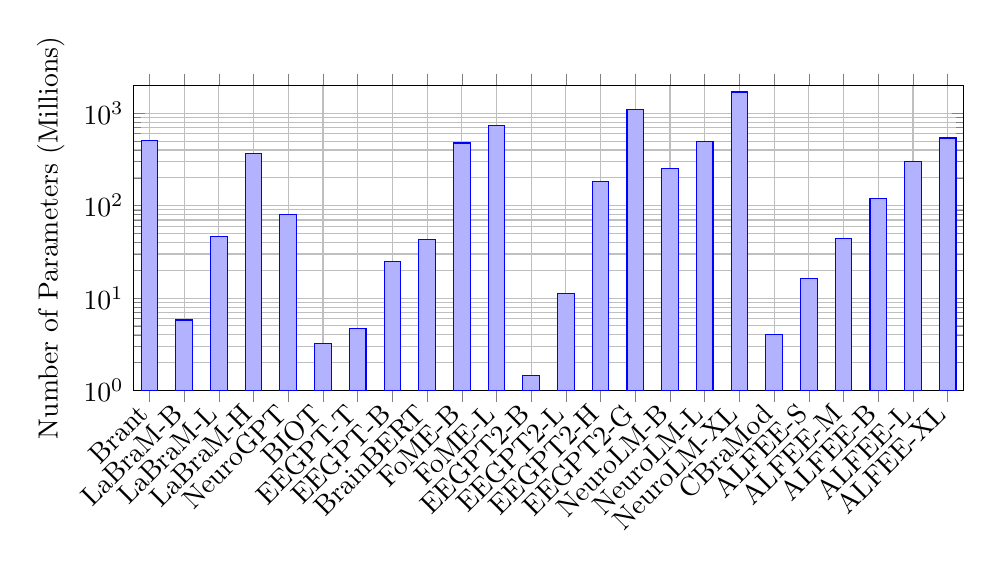
\begin{tikzpicture}
    \begin{axis}[
            ybar,
            width=\linewidth,
            height=0.45\linewidth,
            ylabel={Number of Parameters (Millions)},
            symbolic x coords={
                    Brant,
                    LaBraM-B, LaBraM-L, LaBraM-H,
                    NeuroGPT,
                    BIOT,
                    EEGPT-T, EEGPT-B,
                    BrainBERT,
                    FoME-B, FoME-L,
                    EEGPT2-B, EEGPT2-L, EEGPT2-H, EEGPT2-G,
                    NeuroLM-B, NeuroLM-L, NeuroLM-XL,
                    CBraMod,
                    ALFEE-S, ALFEE-M, ALFEE-B, ALFEE-L, ALFEE-XL
                },
            xtick=data,
            x tick label style={rotate=45, anchor=east},
            ymode=log,
            ymin=1,
            ymax=2000,
            log basis y={10},
            bar width=6pt,
            enlarge x limits=0.02,
            grid=both,
        ]

        \addplot coordinates {
                (Brant,505.69)

                (LaBraM-B,5.8)
                (LaBraM-L,46)
                (LaBraM-H,369)

                (NeuroGPT,79.53)
                (BIOT,3.2)

                (EEGPT-T,4.7)
                (EEGPT-B,25)

                (BrainBERT,43.18)

                (FoME-B,476.3)
                (FoME-L,744.8)

                (EEGPT2-B,1.46)
                (EEGPT2-L,11.29)
                (EEGPT2-H,183.8)
                (EEGPT2-G,1090)

                (NeuroLM-B,254)
                (NeuroLM-L,500)
                (NeuroLM-XL,1696)

                (CBraMod,4.0)

                (ALFEE-S,16.3)
                (ALFEE-M,44.3)
                (ALFEE-B,120)
                (ALFEE-L,300)
                (ALFEE-XL,540)
            };

    \end{axis}
\end{tikzpicture}
